\documentclass[10pt]{report}
\usepackage[centertags]{amsmath}
\usepackage{amsfonts}
\usepackage{amssymb}
\usepackage{amsthm}
\usepackage{newlfont}
\usepackage{graphicx}
%\usepackage[super,sort&compress]{natbib}
%\usepackage[sort&compress]{natbib}
%\usepackage[numbers]{natbib}
\usepackage[authoryear,square]{natbib}

\hfuzz2pt
\newlength{\defbaselineskip}
\setlength{\defbaselineskip}{\baselineskip}
\newcommand{\setlinespacing}[1]%
           {\setlength{\baselineskip}{#1 \defbaselineskip}}
\newcommand{\doublespacing}{\setlength{\baselineskip}%
                           {2.0 \defbaselineskip}}
\newcommand{\singlespacing}{\setlength{\baselineskip}{\defbaselineskip}}
\newcommand{\A}{{\cal A}}
\newcommand{\h}{{\cal H}}
\newcommand{\s}{{\cal S}}
\newcommand{\W}{{\cal W}}
\newcommand{\BH}{\mathbf B(\cal H)}
\newcommand{\KH}{\cal  K(\cal H)}
\newcommand{\Real}{\mathbb R}
\newcommand{\Complex}{\mathbb C}
\newcommand{\Field}{\mathbb F}
\newcommand{\RPlus}{[0,\infty)}
\newcommand{\norm}[1]{\left\Vert#1\right\Vert}
\newcommand{\essnorm}[1]{\norm{#1}_{\text{\rm\normalshape ess}}}
\newcommand{\abs}[1]{\left\vert#1\right\vert}
\newcommand{\set}[1]{\left\{#1\right\}}
\newcommand{\seq}[1]{\left<#1\right>}
\newcommand{\eps}{\varepsilon}
\newcommand{\To}{\longrightarrow}
\newcommand{\RE}{\operatorname{Re}}
\newcommand{\IM}{\operatorname{Im}}
\newcommand{\Poly}{{\cal{P}}(E)}
\newcommand{\EssD}{{\cal{D}}}
\theoremstyle{plain}
\newtheorem{thm}{Theorem}[section]
\newtheorem{cor}[thm]{Corollary}
\newtheorem{lem}[thm]{Lemma}
\newtheorem{prop}[thm]{Proposition}
\theoremstyle{definition}
\newtheorem{defn}{Definition}[section]
\theoremstyle{remark}
\newtheorem{rem}{Remark}[section]
\newcommand{\field}[1]{\mathbb{#1}}
\newcommand{\C}{\field{C}}
\newcommand{\R}{\field{R}}
\newcommand{\script}[1]{\mathcal{#1}}
\DeclareSymbolFont{AMSb}{U}{msb}{m}{n}
\DeclareMathSymbol{\dbln}{\mathalpha}{AMSb}{"4E}
\DeclareMathSymbol{\dblp}{\mathalpha}{AMSb}{"50}
\DeclareMathSymbol{\dblz}{\mathalpha}{AMSb}{"5A}
\DeclareMathSymbol{\dblr}{\mathalpha}{AMSb}{"52}
\DeclareMathSymbol{\dblt}{\mathalpha}{AMSb}{"54}
\DeclareMathSymbol{\dblq}{\mathalpha}{AMSb}{"51}
\DeclareMathSymbol{\dbln}{\mathalpha}{AMSb}{"4E}
\DeclareMathSymbol{\dblf}{\mathalpha}{AMSb}{"46}
\DeclareMathSymbol{\dblc}{\mathalpha}{AMSb}{"43}
\DeclareMathSymbol{\dbld}{\mathalpha}{AMSb}{"44}
\newcommand{\fall}{\; \forall \;}
\newcommand{\exts}{\; \exists \;}
\newcommand{\st}{\; \ni \;}
\newcommand{\mbf}[1]{\mathbf{#1}}
\newcommand{\binomial}[2]{\biggl( \begin{array}{c}  #1 \\ #2  \\ \end{array} \biggr) }
\newcommand{\fderiv}[2]{ \frac{d}{ d #1} \: #2}
\newcommand{\sderiv}[2]{ \frac{d^2}{ d^2 #1} \: #2}
\newcommand{\pfderiv}[2]{ \frac{\partial}{ \partial #1} \: #2}
\newcommand{\psderiv}[2]{ \frac{\partial^2}{ \partial^2 #1} \: #2}
\newcommand{\mat}[1]{\mathbf{#1}}
\numberwithin{equation}{section}
\renewcommand{\theequation}{\thesection.\arabic{equation}}
\title{Numerical Linear Algebra Project: OSU MATH 5603 }
\author{Bruce B. Campbell}
\begin{document}
%\def\baselinestretch{1}
\setlinespacing{1.25}
\newcommand{\footn}[1]{\footnote{\hspace{0.1cm}\parbox[t]{13.25cm}{#1}}}
\maketitle
\section*{Spectral Methods in Data Science}

There are lots of applications of Numerical Linear Algebra in data science. One could easily make the case that the Singular Value Decomposition (SVD) and iterative eigensolvers are some of the most important algorithms in industry. Principal Component Analysis (PCA) is one of the most common spectral methods in data science; using the SVD to resolve important directions in data space that have the most variance. PCA is useful if the variance describes something were interested in, as it can tell us what that direction is and provide a transformation of the data to a low dimensional space.   

In this paper we are going to explore some of the applications of eigensolver algorithms to a particular type of clustering algorithm in data science called spectral clustering. The idea behind spectral clustering is to transform a data set with $n$ samples and $m$ features, $X \in \dblr^{n,m}$ to a graph that we can operate on to resolve different clusters in the data. 

The rest of this paper is organized as follows
\begin{itemize}
\setlength\itemsep{-0.5em}
    \item {Definitions}
    \item {Overview of Spectral Clustering}
    \item {Observations from clustering synthetic data}
\end{itemize}

\section*{Definitions}
We try to keep with these conventions in our code as well. Let $X \in \dblr^{n,m}$ be our data set.  $G$, a graph is a collection of edges and vertices $(G=(E,V)$. $u \; v$ are edges and if they are connected we write $u \sim v$ We write $|V|$ , $|E|$ for the number of vertices and edges respectively. $A \in \dblr^{|V| \times |V| }$ is a graph adjacency matrix; $A_{u,v} = 1 : u \sim v$. $\rho(x_i,x_j)$ will denote a metric or similarity function. We write $K_{\rho}(x_i,x_j)$ for the similarity matrix induced by the similarity measure $\rho$. Sometimes we don't distinguish between $K$ and $A$.  Indeed, if $A$ is the complete graph and it's a weighted graph weighted by similarity - then $K=A$.  Lastly we'll be dealing with diagonal matrices of degree or weight sums - we denote $d_v$ to be the degree of $v$ in the unweighted case or the sum of the sum of the weights $d_v = \sum_{u} K(x_v,x_u)$  in the weighted case.   

\section*{Overview of Spectral Clustering}

There are many variants of the spectral clustering algorithm. There's a rich history of the techniques, some originating in the parallel solution of PDE's where it's called graph partitioning.  We'll see more about graph cuts below. The basic idea of spectral clustering is to use the eigenvectors of a similarity matrix for the data to perform dimension reduction to a low dimensional space where clustering is performed.  If we're interested in regression or classification - that can also be done in the low dimensional space. 

There are two key ingredients to forming the affinity matrix; a distance function, and a convention for which pairs to consider.  If all or too many pairs are compared, sparse methods might not be possible.  We can include $k$ nearest points, all points within $\epsilon$ of a sample $x_i$, or some other criteria. For instance when working with spatial data, the diffusion can be done on a graph formed by a tessellation of the locations.  This is exactly how numerical solutions of heat diffusion is done. In spatial biology applications a cell communication distance can be used to form the graph where the distance is some reasonable measure of inter-cellular communication - then all cells within $\epsilon$ of a sample $x_i$ will be connected. This creates graphs of communicating cell networks. 

Spectral graph theory takes lots of insights from geometry.  Discrete analogues of isoperimetry results and heat flow on manifolds are just a few examples.  The normalized graph Laplacian is used to aid in consistency between spectral geometry and stochastic processes.  The best reference for background material is \cite{chung1997spectral}. 

We generally consider connected graphs $G = (E,V)$ in this work, in which case we can define the normalized graph Laplacian as $\mathcal{L} = T^{\frac{1}{2}} L T^{\frac{-1}{2}} = I - T^{\frac{1}{2}} A T^{-\frac{1}{2}}$, where $A$ is the adjacency matrix, $L$ is defined by

\begin{equation*}
L(u,v)  = \Biggl\{
\begin{array}{cc}
 d_v & :\; u=v \\
 -1  & : u\sim v  \\
 0   & : u \nsim v  \end{array}
\end{equation*} and
$T = diag\{d_1, \cdots , d_n\}$ where $d_v$ is the degree of vertex $v$ or the sum of weights as described above.

$\mathcal{L}$ is a difference operator on the space of functions $g \in \dblr^{|V|}$

\begin{equation*}
 \mathcal{L} g  = \frac{1}{\sqrt{d_u}} \sum\limits_{v : u \sim v} ( \frac{g(u)}{\sqrt{d_u}} -  \frac{g(v)}{\sqrt{d_v} } )
\end{equation*}

\begin{eqnarray}
Vol (G) = \sum\limits_{v \in V}^{d_v} = Tr(T) \\
\sigma(\mathcal{L}) \in \dblr^+ \\
ker ( \mathcal{L} ) = span\{ T^{\frac{1}{2}} 1 \}
\end{eqnarray}

This is the same difference operator ( up to the scaling by T ) that describes the coupled mass spring system.  It is the discrete analog of the continuous Laplacian $\Delta f=\sum_{i=1}^n \frac{\partial^2 f}{\partial x_i^2}$ which has eigenfunctions $f(x)=e^{j n x}$ We know from PDE's that the boundary of the domain of the operator determines it's fundamental modes.  This is still the case in the discrete setting. We'll see below that the graph Laplacian has eigenvectors that correspond to high and low frequencies. 

There are many nice properties of the Laplacian matrix. It's symmetric, positive semi-definite and diagonally dominant. The implications of which are that the eigenvalues are real and non negative. When a matrix has a large condition number it can be pre-conditioned for better performance in solvers, particularly for iterative solvers. The multiplication of $L$ on the left and right by $T$ might be seen as a form of Jacobi (diagonal) pre-conditioning. We know the matrix is singular, but it might help with eigenvalue condition numbers. We perform some experiments below to investigate this. 

Notice we have defined a discrete version of the traditional Laplacian.  There are many interesting comparisons between the discrete setting and continuous geometry. We will see later, the data set we analyze has been prepared to mirror the setting of heat conduction and capture some of the aspects of isoperimetry.

We can now describe the basic steps of spectral clustering.  We stick with the method defined in \cite{NIPS2001_801272ee}

\begin{itemize}
\setlength\itemsep{-0.5em}
    \item Calculate similarity matrix A
    \item Calculate Laplacian L
    \item Calculate first k eigenvectors $U_k$
    \item Using $U_k(i,j)$ as embedded feature values, cluster in $\dblr^k$
\end{itemize}

Consider the case that we have $l$ classes which are completely dissimilar. If our data is arranged the right way - this means our similarity matrix will be block diagonal. We can then make some nice statements about the spectrum and eigenspaces - namely that they are the union of the blocks. This is theorem 5.2.10 and problem 5.2.20 in \cite{watkins2004fundamentals}.  Now suppose we 'peturb' the inter-class similarity with some noise.  We call this class cross-talk in the accompanying Matlab code. We can use the spectral gaps $| \lambda_i - \lambda_j |$ to analyse the stability of the spectrum and eigenspaces to perturbations. 

Before we introduce our data sets and analysis results it's worth mentioning an important relationship between $G=(E,V)$ and $A$.  If we specify a random walk on $V$ with probabilities $A_{u,v}$, then the mixing time of this random walk is related to the second eigenvalue governs the mixing time.  We can imagine the amount of cross talk is the measure of mixing between classes. One of our aims is to demonstrate this experimentally. 

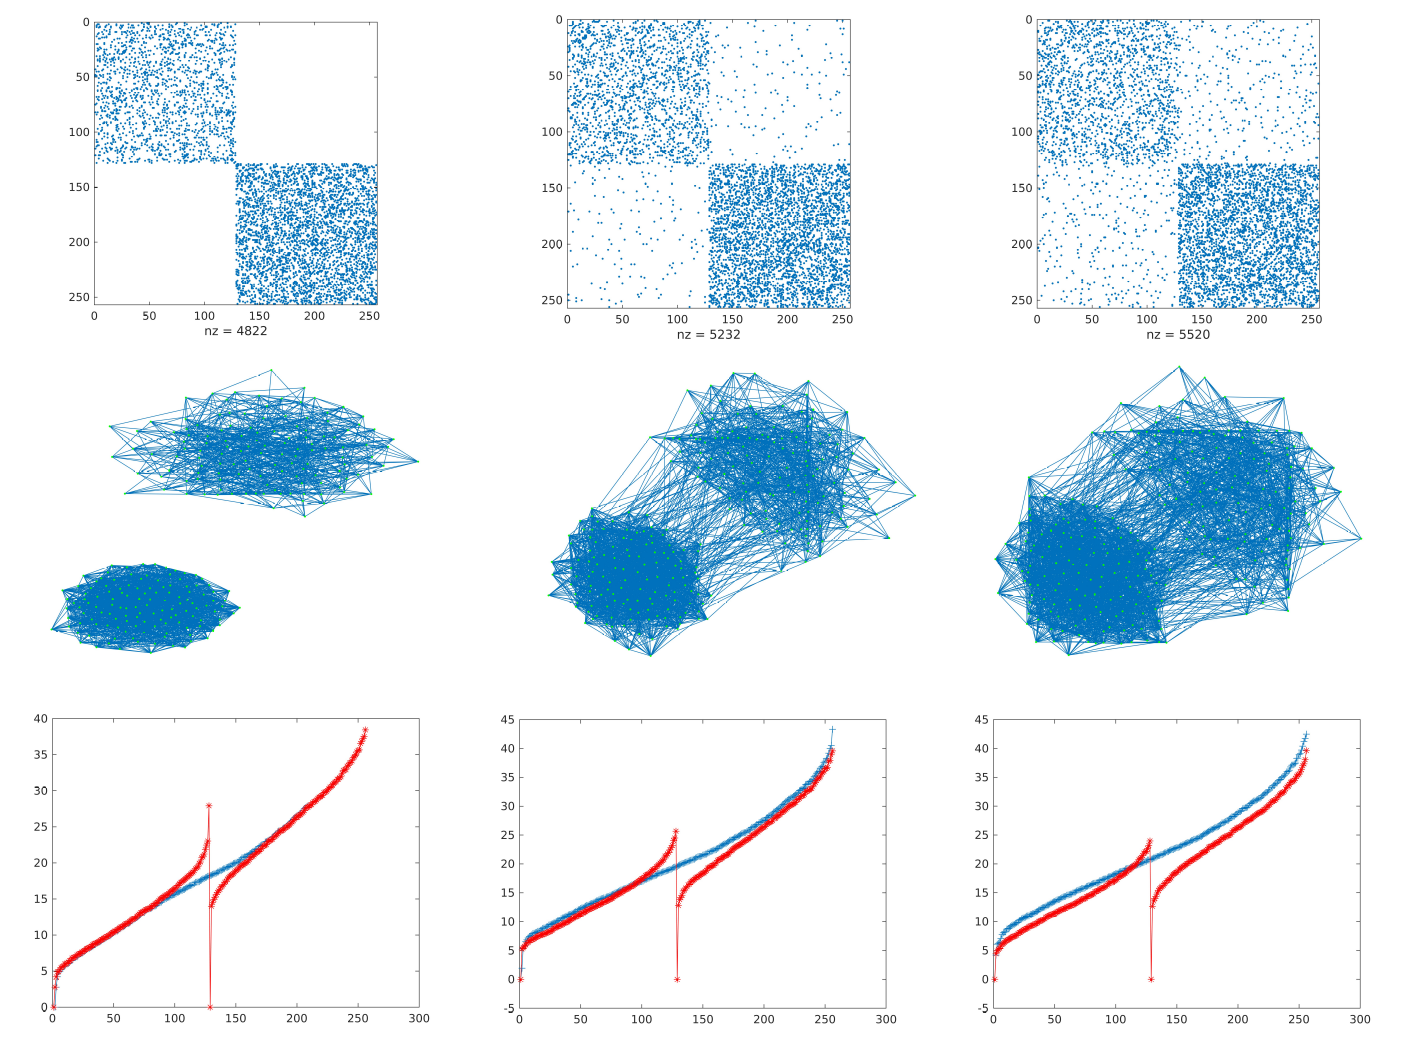
\includegraphics[width=6in,height=6in]{images/2class_gap.png}

In the figure above we have collected a few examples of a two class scenario.  We plotted $\mathcal{L}$, $G$, and the last row is the 2 spectra of the diagonal blocks in red aligned to the spectrum of the full matrix in blue.  The data above for the adjacency matrices $A$ is generated randomly see our Matlab code \cite{git_repository}.  

Remember $\mathcal{L}$ is singular with eigenvector $T^{\frac{1}{2}} 1$.  This is also true for the block diagonal components.  We see good agreement on the spectrum being the union of the components of the blocks when there is no to little crosstalk. On the far right, the union of the spectrum of diagonal blocks is starting to diverge from the spectrum of the full matrix.  This is interesting.  We calculated the eigengap between 0 and the first non-zero eigenvalue for these Laplacians

\begin{table}[h!]
\begin{tabular}{ll}
crosstalk probability & eigengap             \\
\hline
0                     & 3.73034936275466e-14 \\
0.0100000000000000    & 1.93400161800437     \\
0.0200000000000000    & 4.20076779565674     \\
0.0300000000000000    & 4.65155396750515     \\
0.0400000000000000    & 7.85252158678672     \\
0.0500000000000000    & 9.26918323946276     \\
0.0600000000000000    & 9.96142891808756     \\
0.0700000000000000    & 10.9737931514795     \\
0.0800000000000000    & 11.9802338078632     \\
0.0900000000000000    & 12.6376406303656    
\end{tabular}
\end{table}

We see the relationship between the crosstalk and the eigengap makes intuitive sense and is consistent with the Markov chain interpretation of $A$.  As crosstalk increases we see from the graphs above that the random walk on vertices will be able to cross to other clusters.  The more cross talk, the more mixing, and thus the faster convergence to stationarity. 

Next we take a synthetic data set through the spectral clustering process up to the calculations of the eigenvalues and eigenvectors. Again see our github repository for the code to replicate the figures and data. 

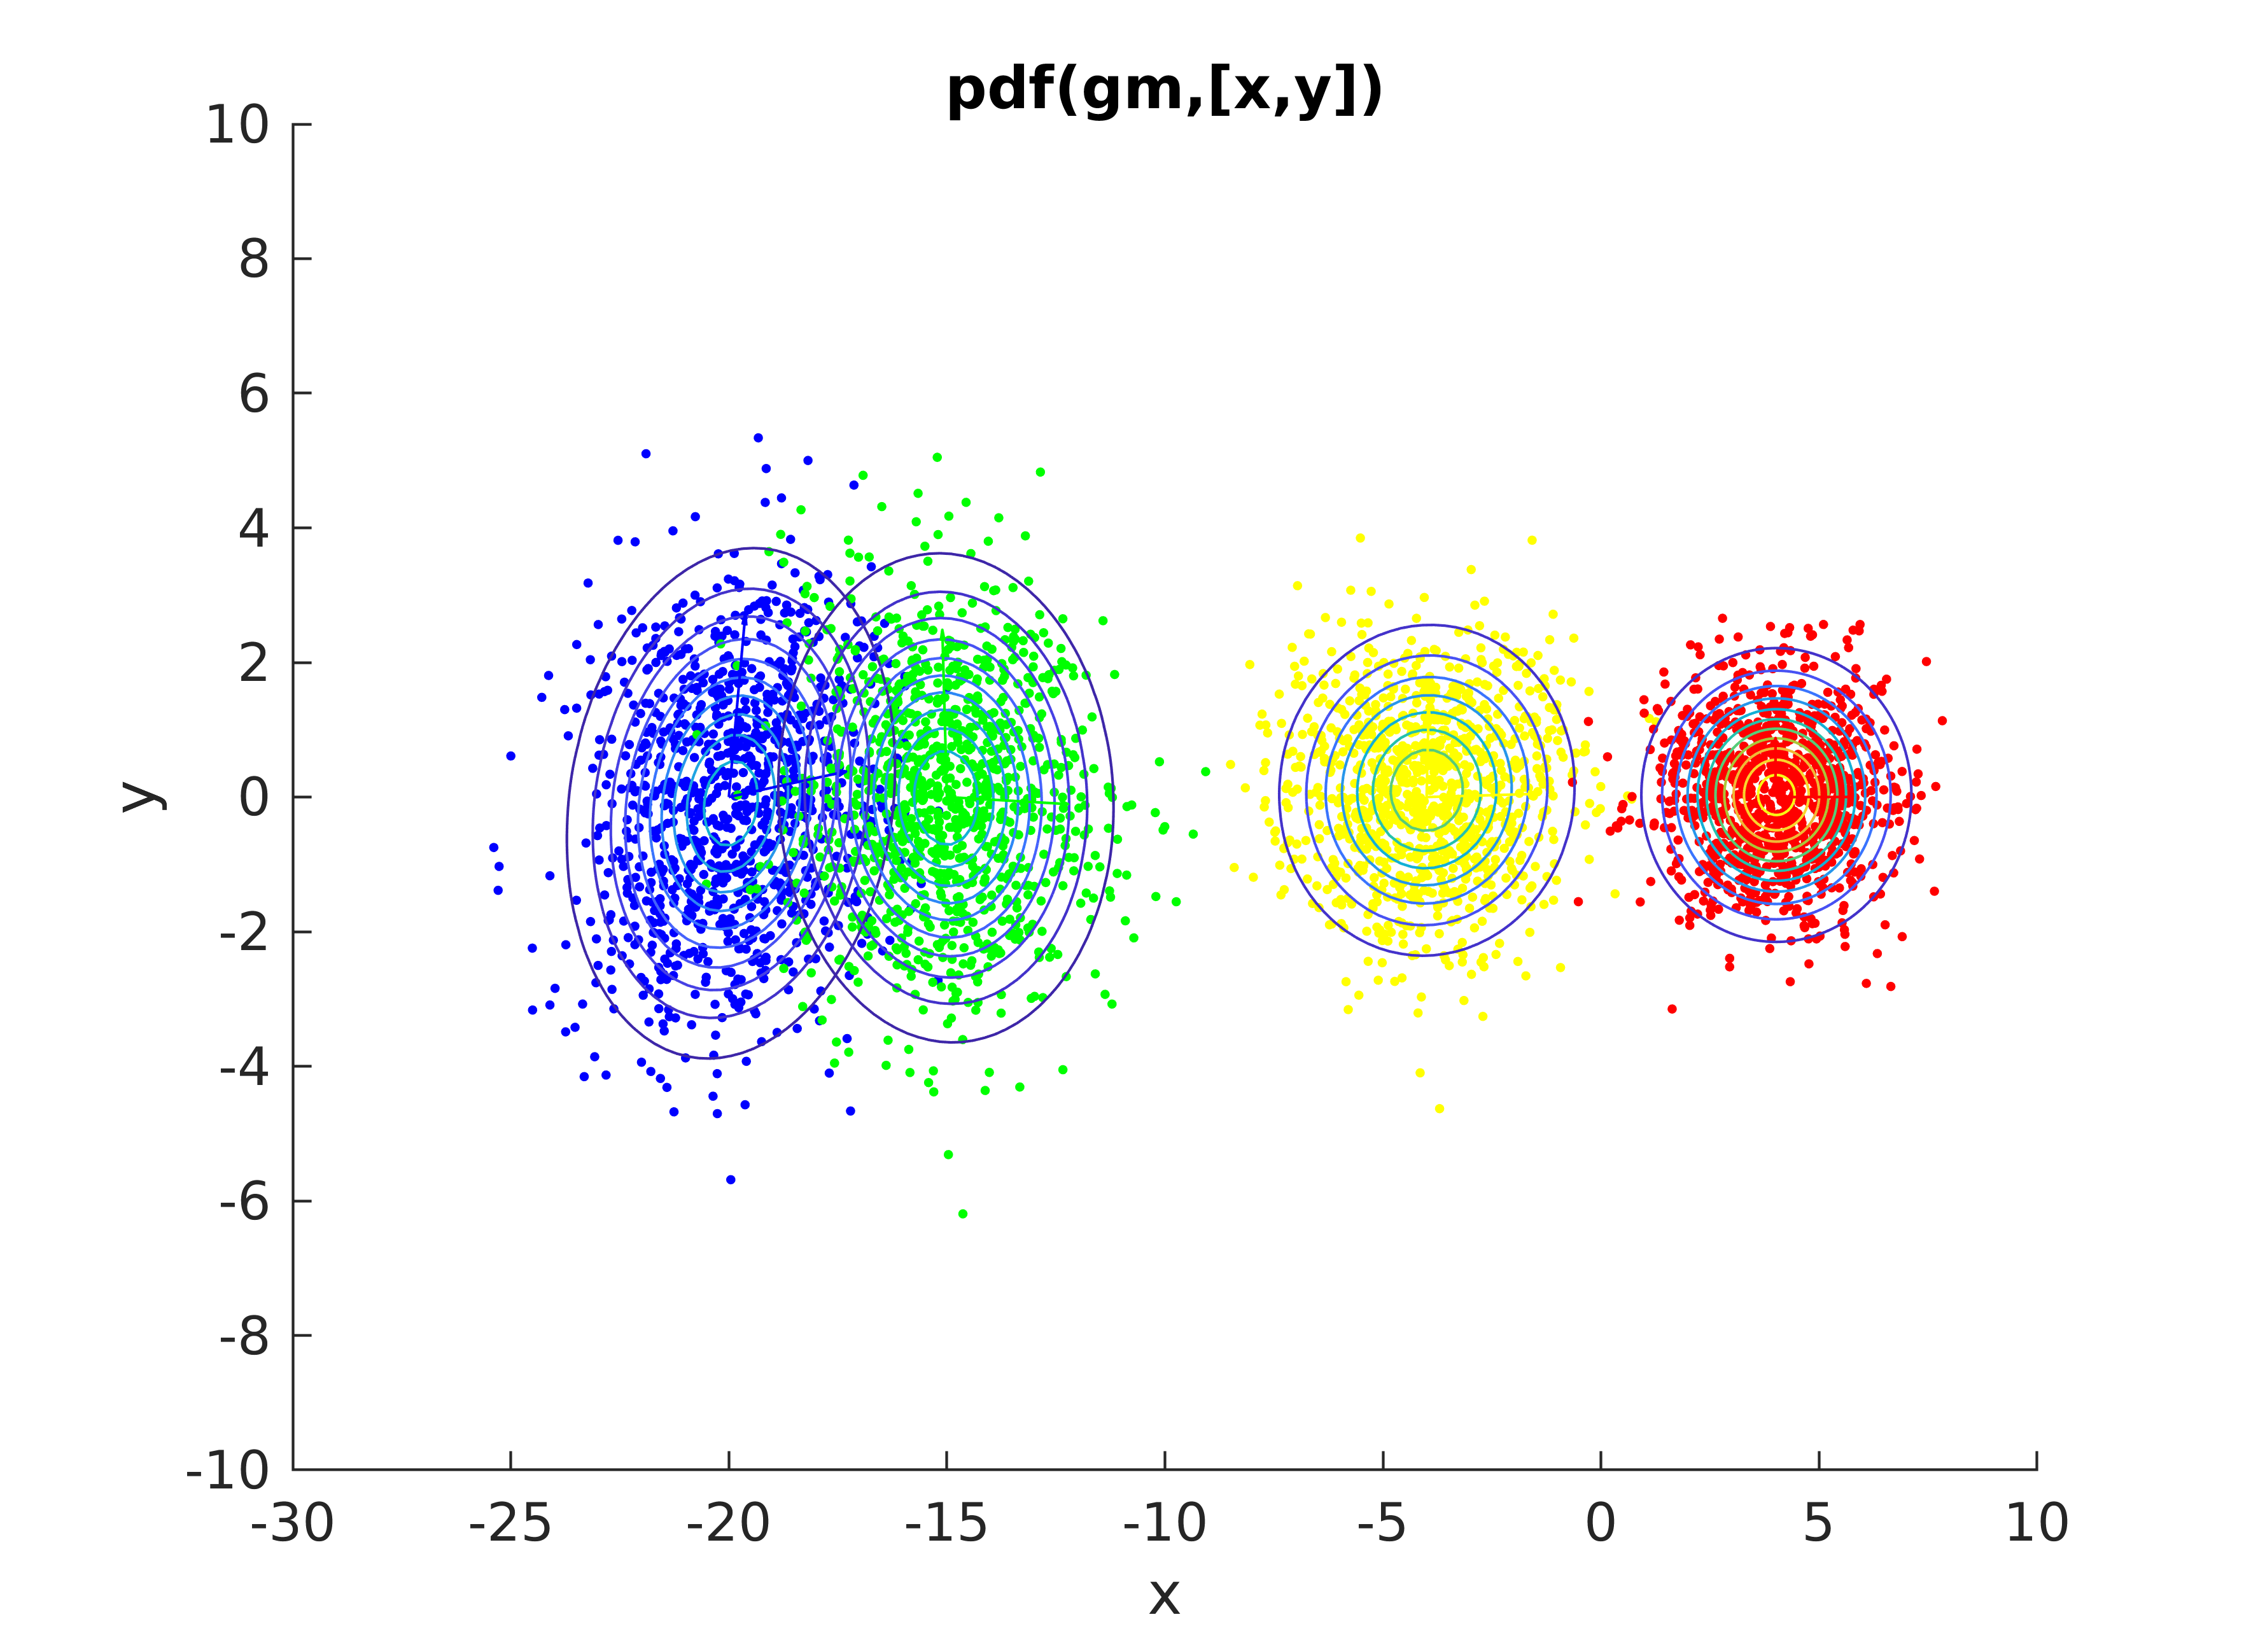
\includegraphics[width=5in,height=4in]{images/4class.png}
This data was designed to have both noise (outliers) and true crosstalk. The data is a sample from a mixture of four bivariate random normal variables.  Data is not usually given to us in such a nice organized format. To convince ourselves of the utility of the approach in the code we rotate the data in a random direction, and we permute both the rows and columns randomly. The effect of this on the adjacency matrix is below. 

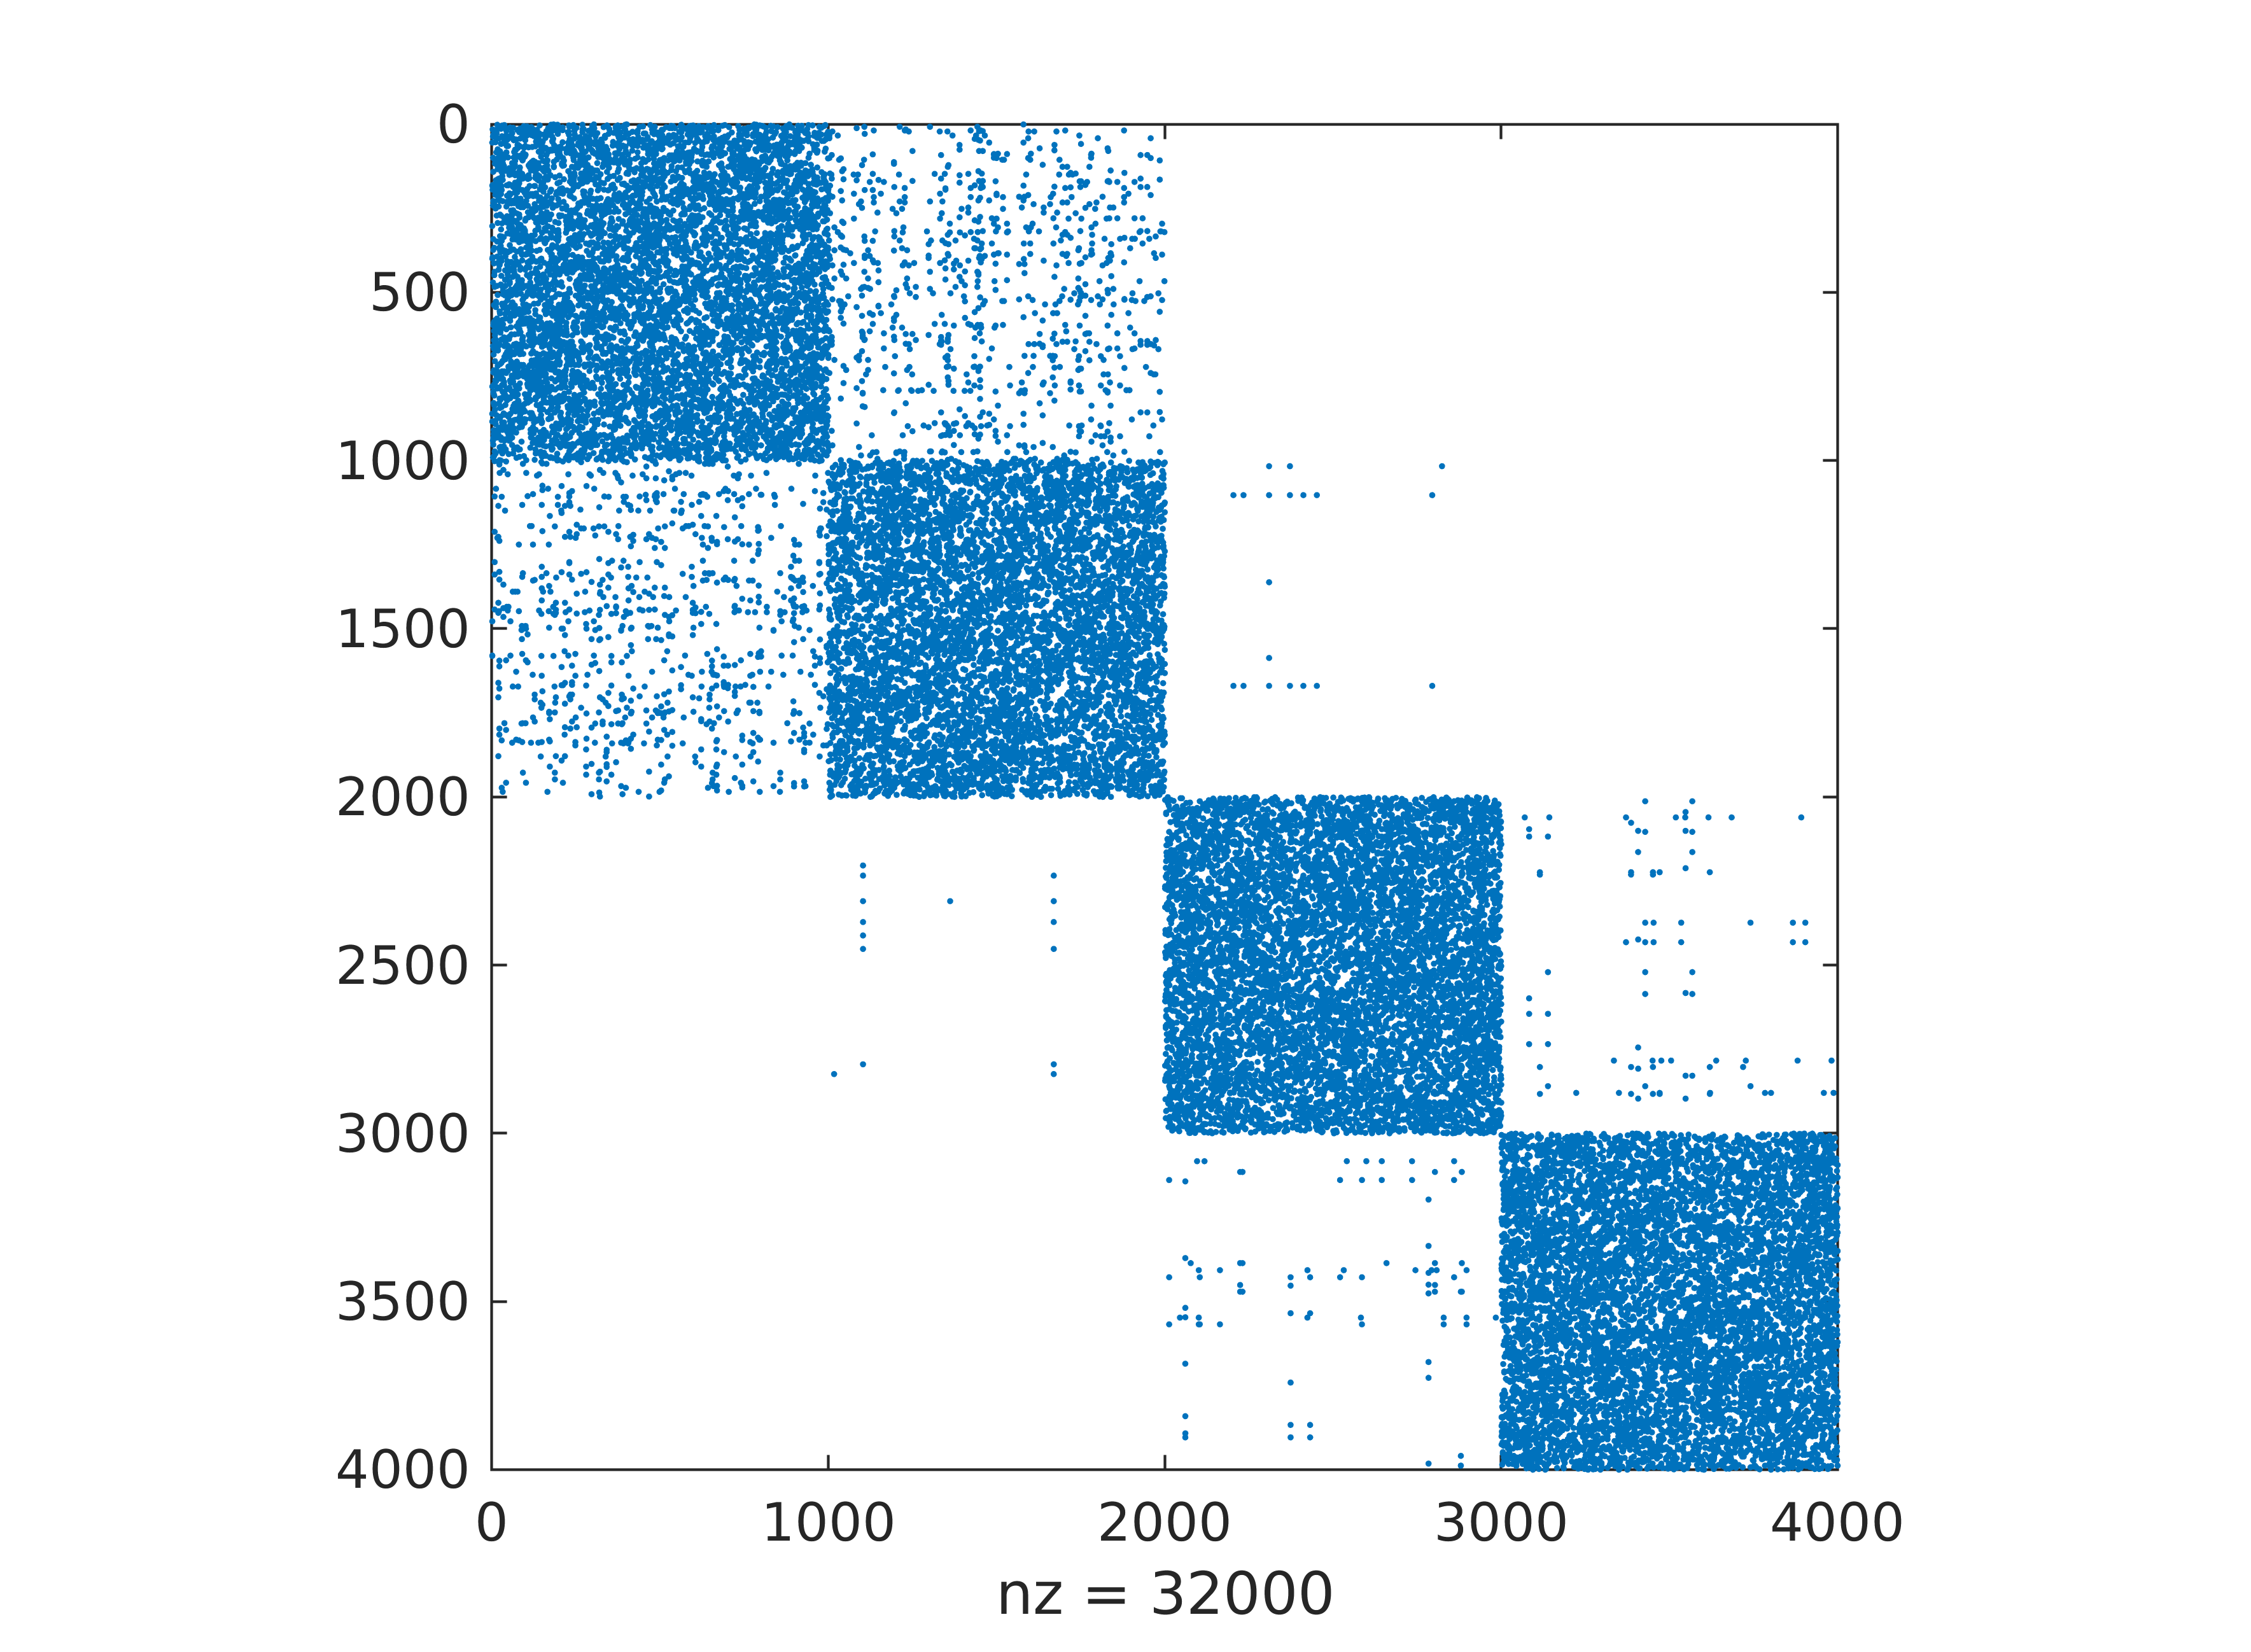
\includegraphics[width=3in,height=3in]{images/spy.png}
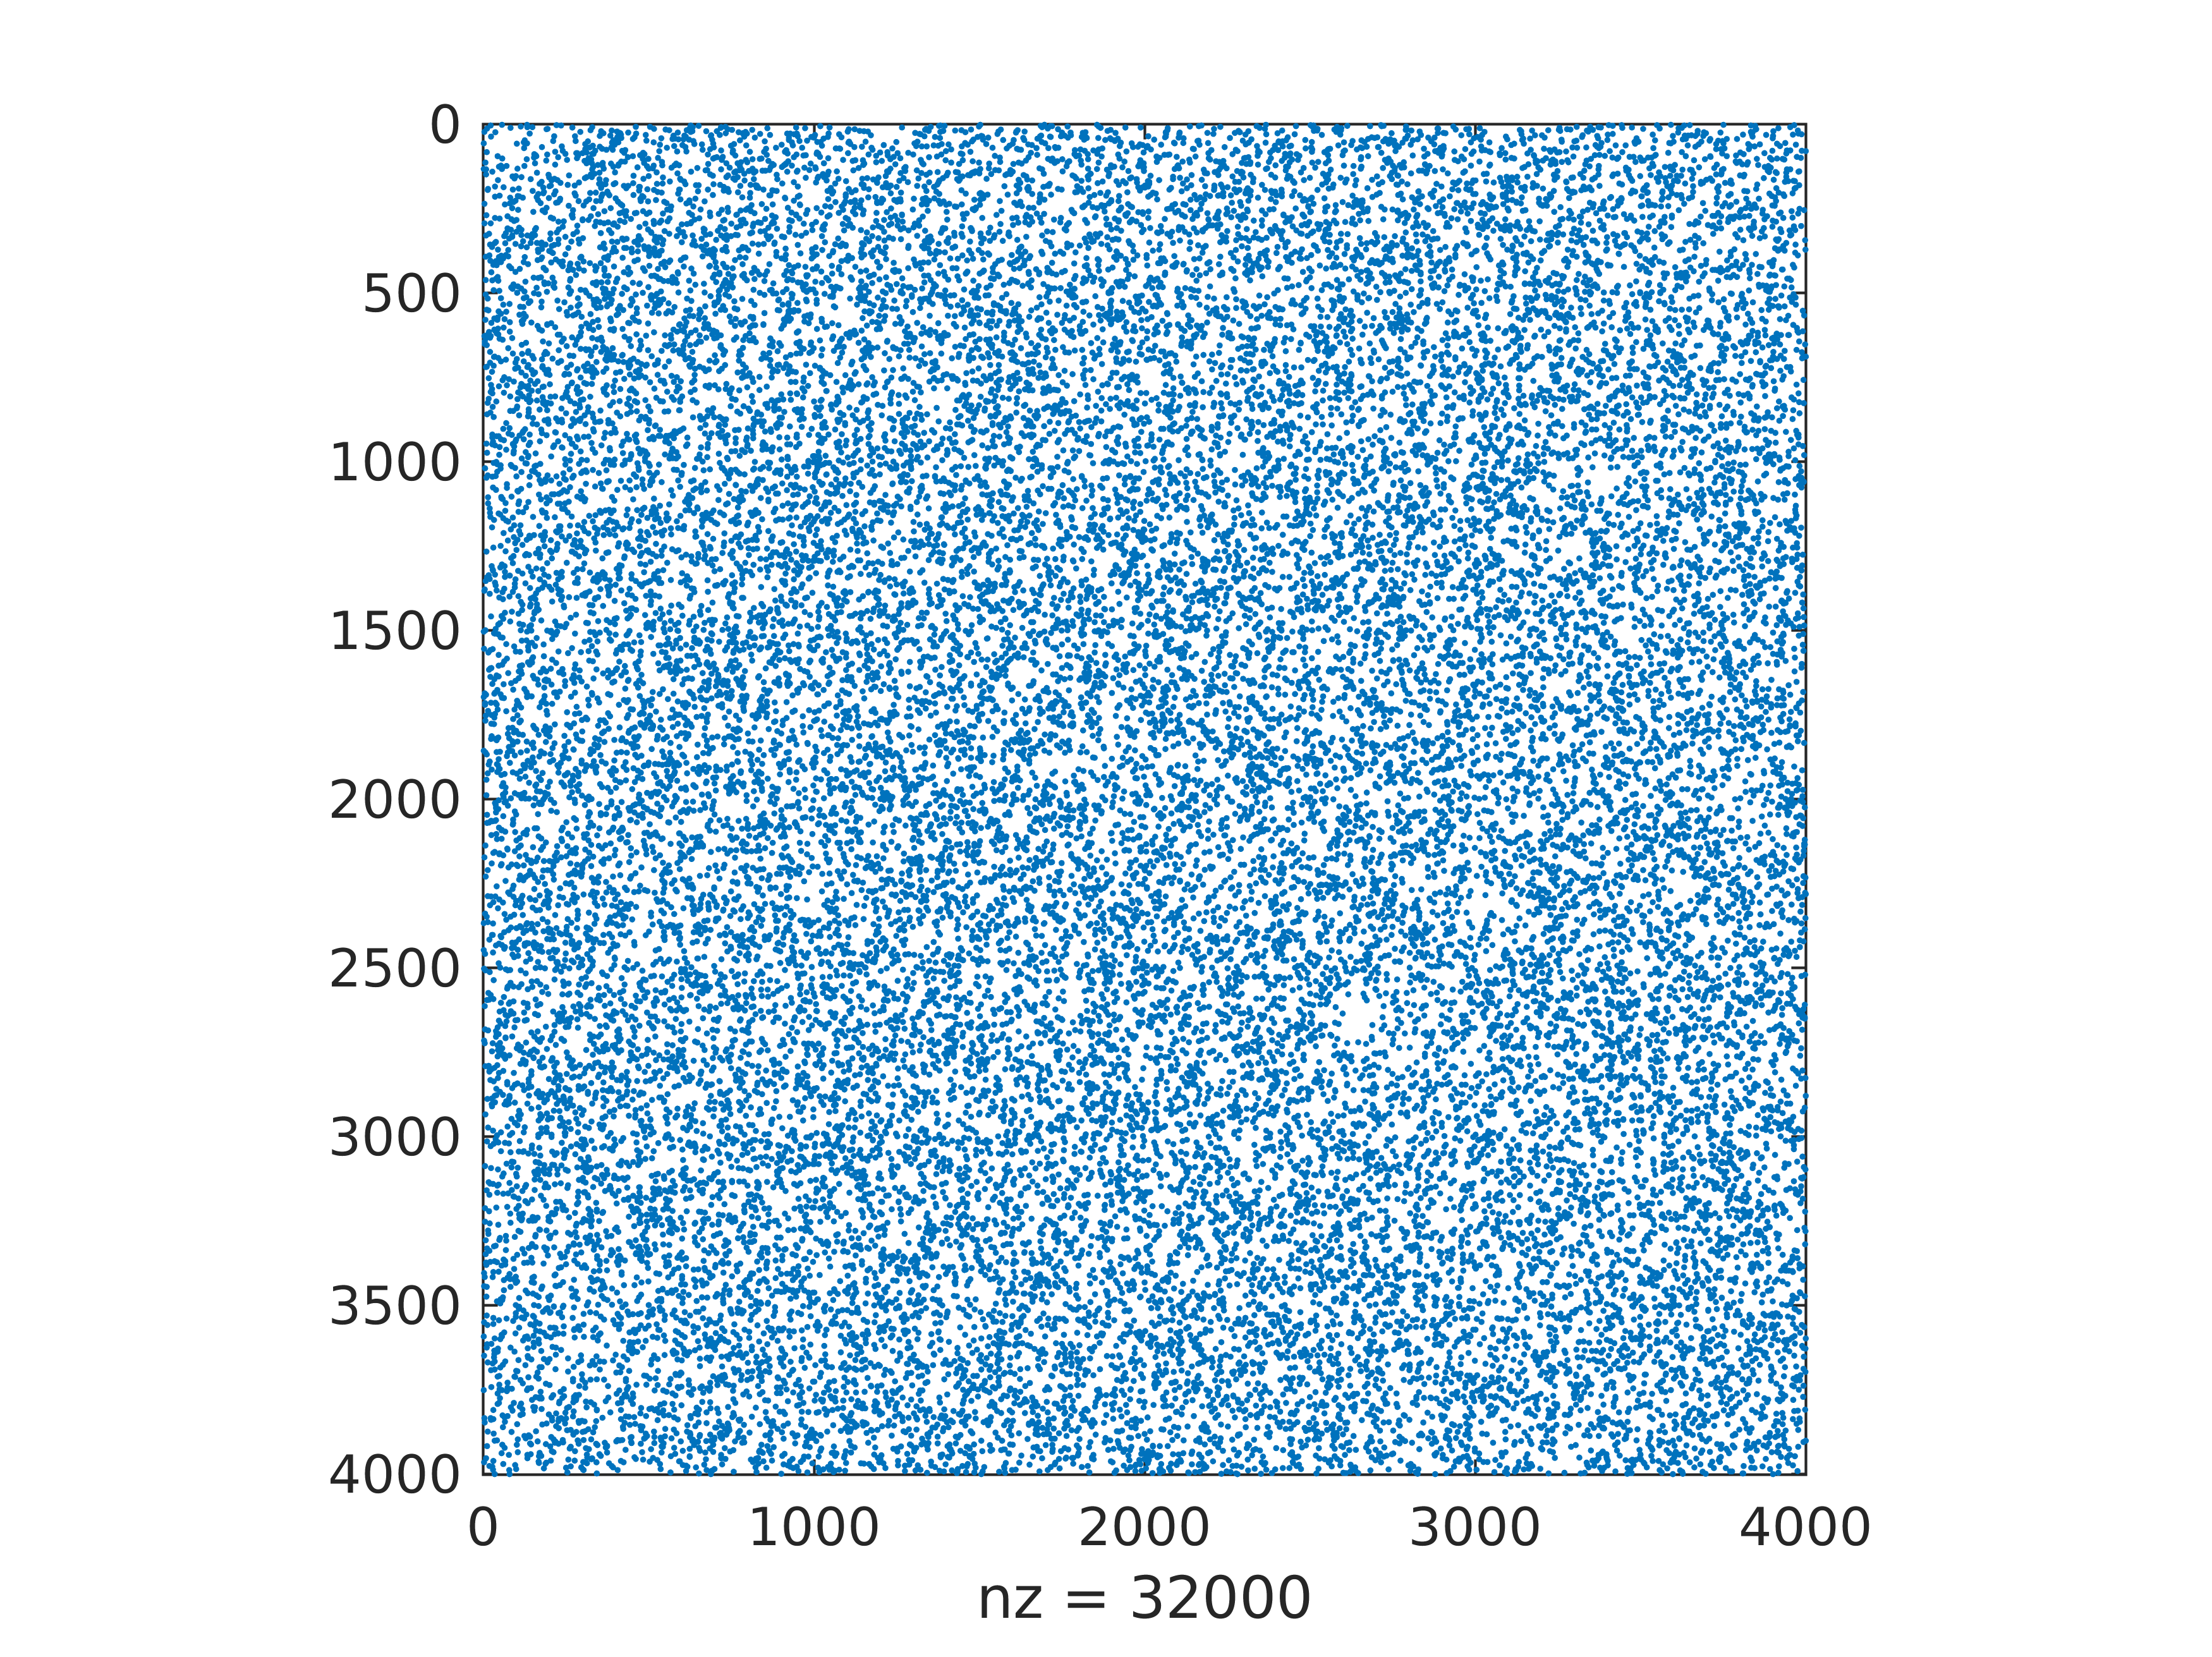
\includegraphics[width=3in,height=3in]{images/spy_randomized.png}
Data analyzed in practice usually arrives out of order, and with no indications which are the important directions. Spectral clustering can help identify underlying hidden structure.  Our data is 2 dimensional but the technique works well in high dimensions.  

We chose to use a nearest neighbor approach for calculating $A$. We experimented with using the Gram matrix $X^T X$ and an adaptive approach based on neighborhoods that provides more connections where the data is more dense and got similar results. Below are the first few eigenvectors for the graph Laplacian of our synthetic data.  

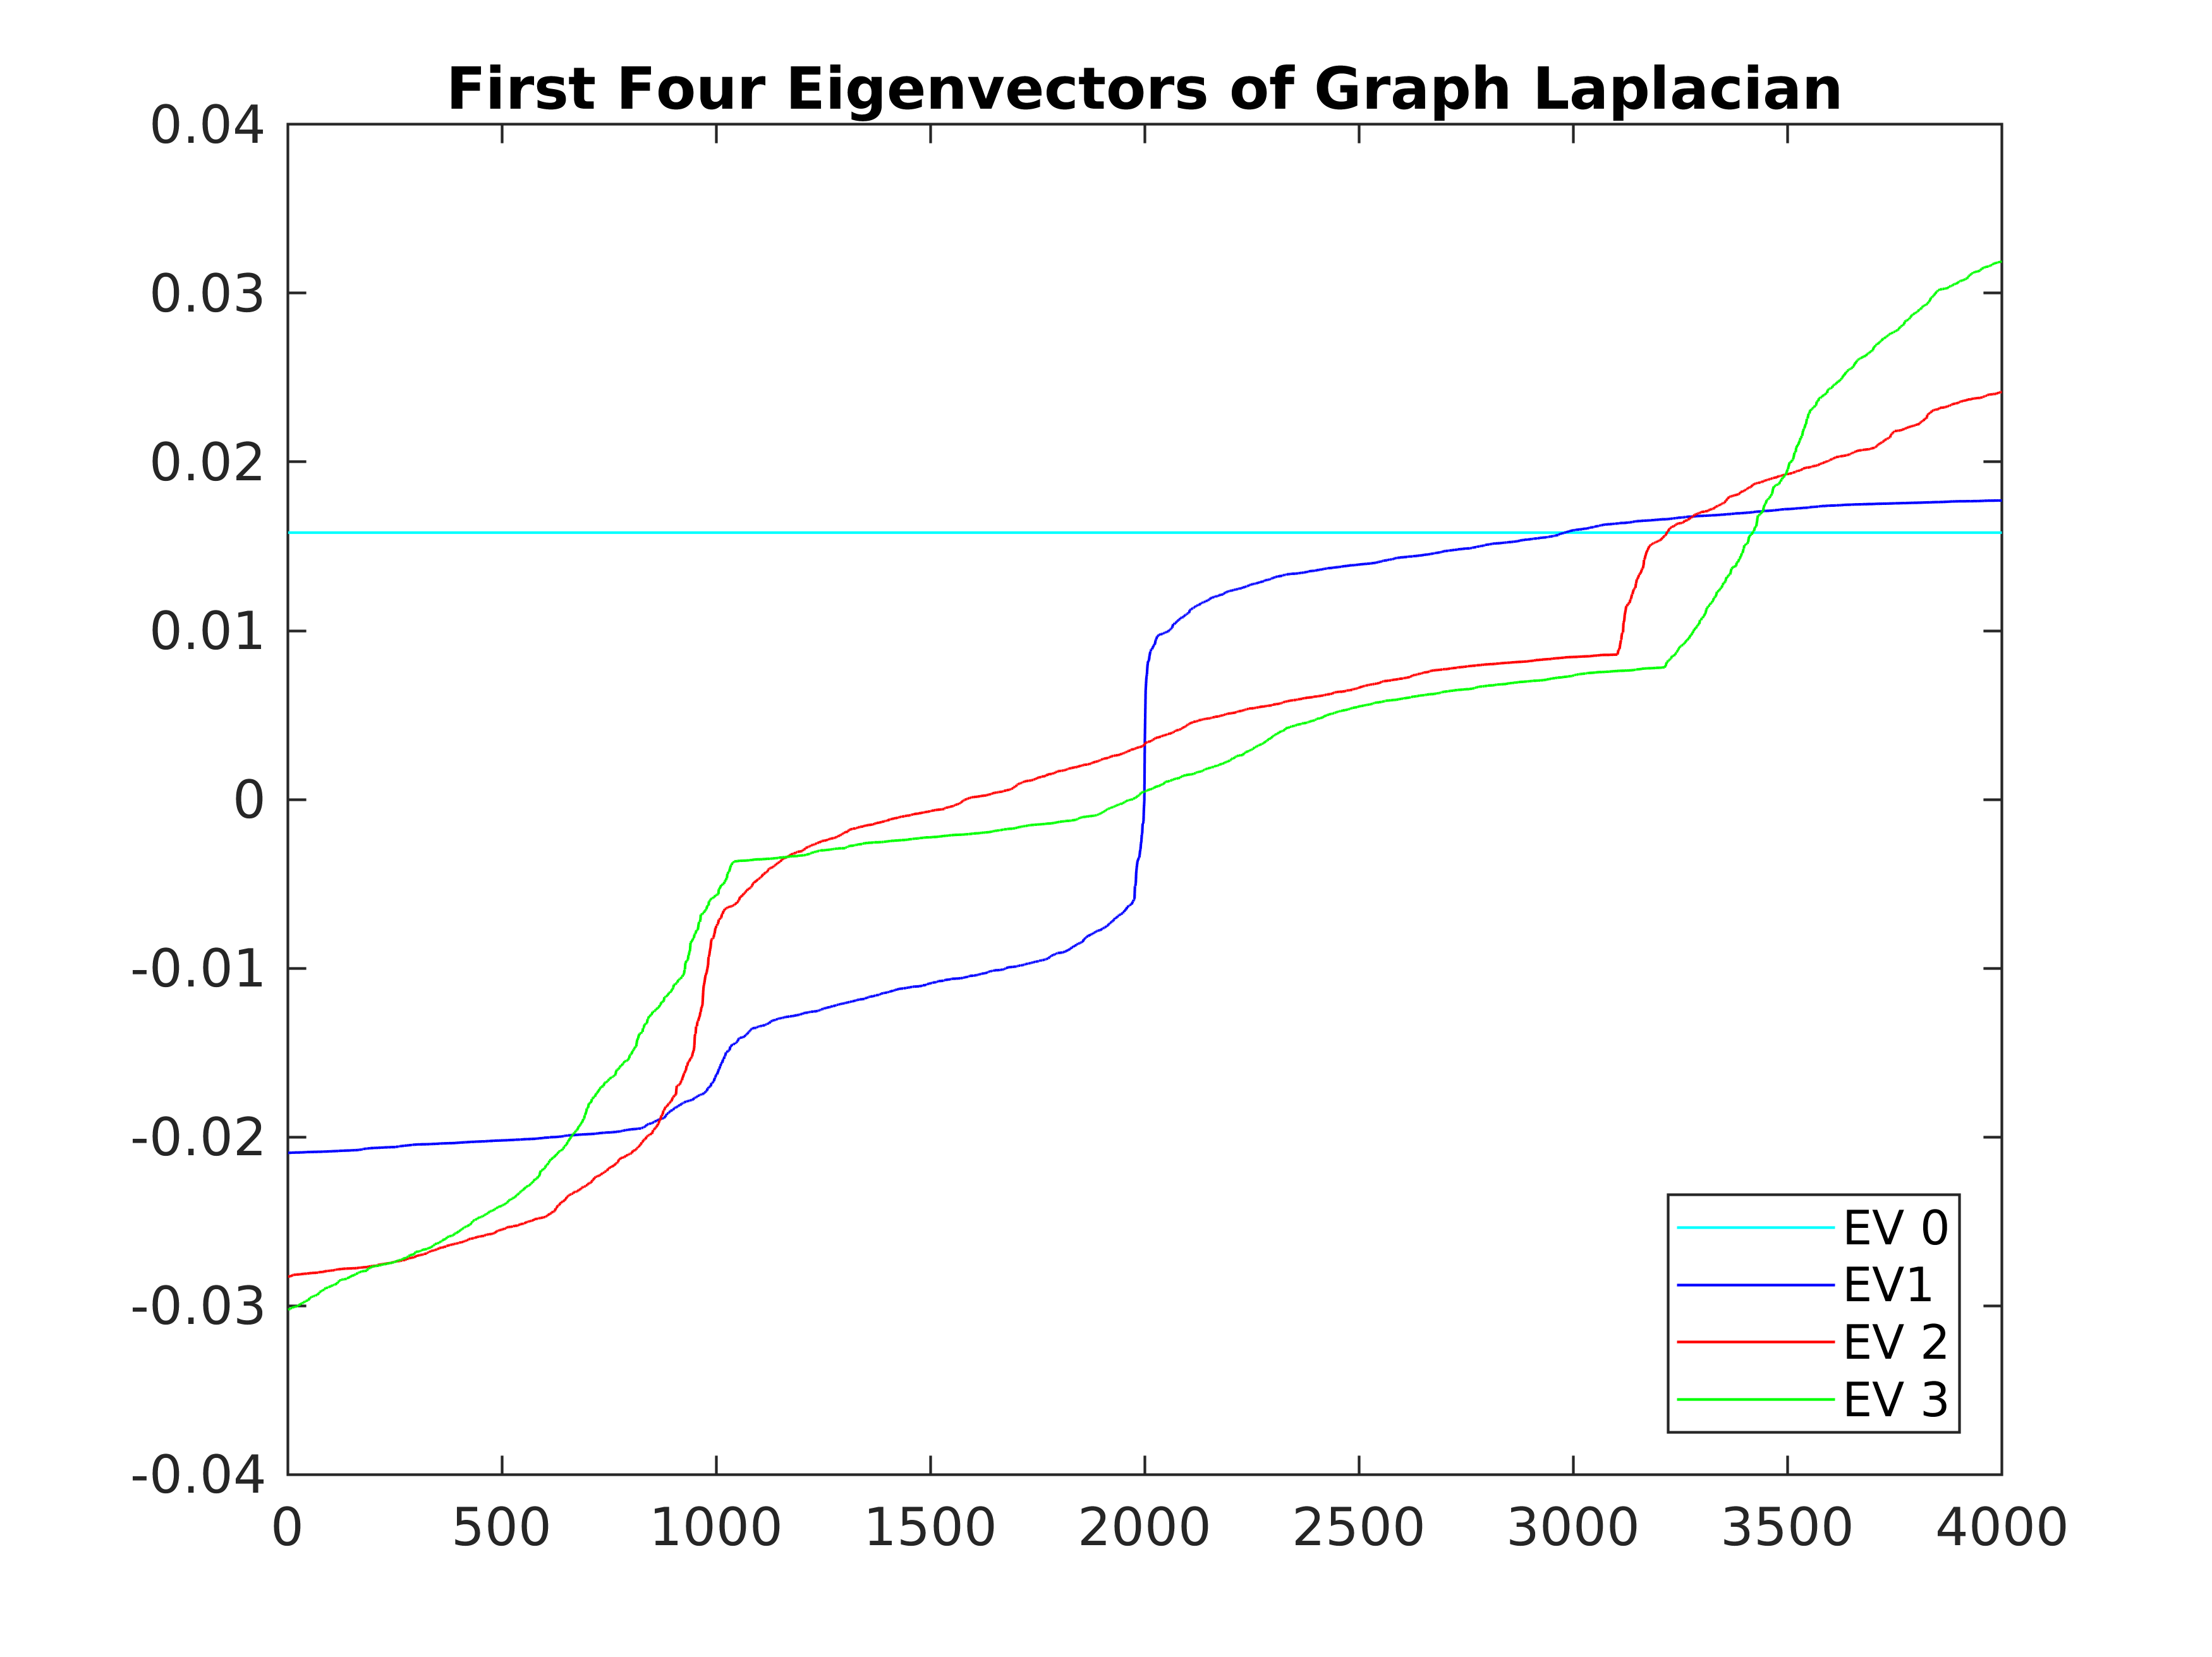
\includegraphics[width=3in,height=3in]{images/eigenvecs.png}

We see the values of the eigenvectors capture the differences in classes nicely. The same diagram is presented for the two class data that has a low crosstalk. We see the second eigenvector separates the data based on sign alone.  

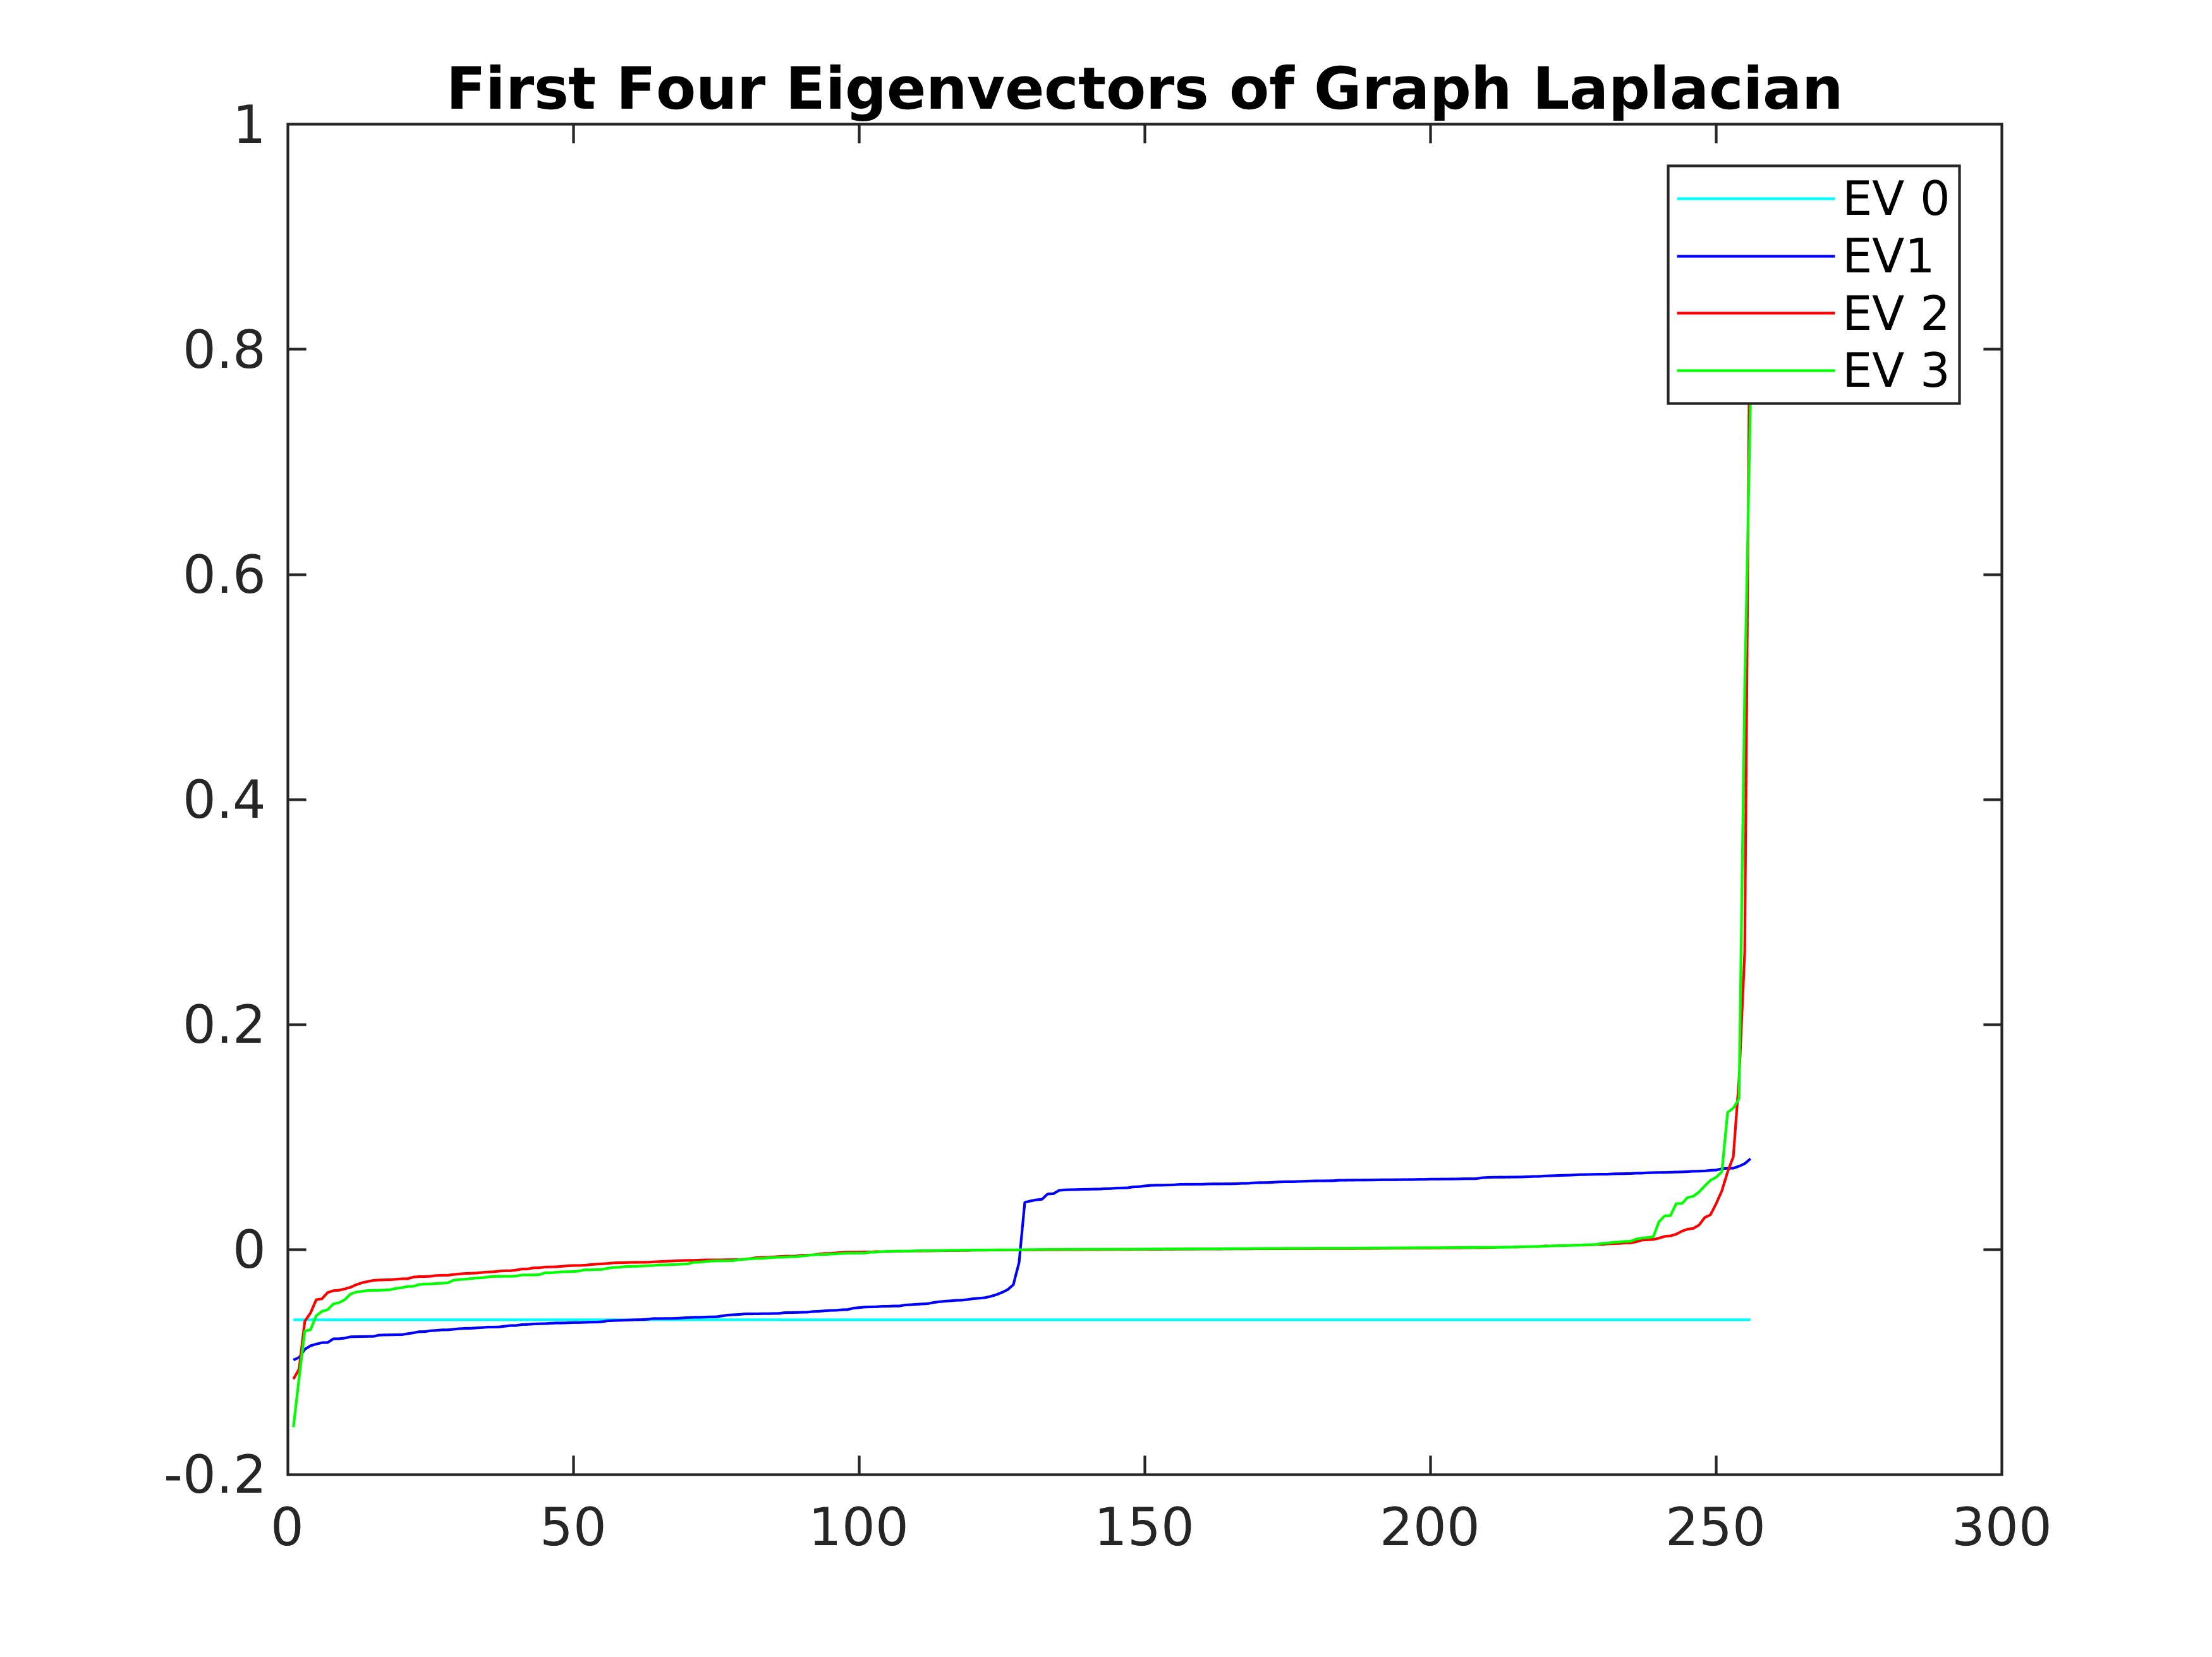
\includegraphics[width=3in,height=3in]{images/EigenVectors_P1_0.100000_P2_0.200000_crosstalk_0.010000_gap_2.329507.jpg}






























\setlinespacing{1.1}
\bibliographystyle{plainnat}
\bibliography{thebibliography}
\end{document}
